\documentclass{beamer}
\usepackage[utf8]{inputenc}

\usetheme{Madrid}
\usecolortheme{default}
\usepackage{amsmath,amssymb,amsfonts,amsthm}
\usepackage{txfonts}
\usepackage{tkz-euclide}
\usepackage{listings}
\usepackage{adjustbox}
\usepackage{array}
\usepackage{tabularx}
\usepackage{gvv}
\usepackage{lmodern}
\usepackage{circuitikz}
\usepackage{tikz}
\usepackage{graphicx}

\setbeamertemplate{page number in head/foot}[totalframenumber]

\usepackage{tcolorbox}
\tcbuselibrary{minted,breakable,xparse,skins}



\definecolor{bg}{gray}{0.95}
\DeclareTCBListing{mintedbox}{O{}m!O{}}{%
  breakable=true,
  listing engine=minted,
  listing only,
  minted language=#2,
  minted style=default,
  minted options={%
    linenos,
    gobble=0,
    breaklines=true,
    breakafter=,,
    fontsize=\small,
    numbersep=8pt,
    #1},
  boxsep=0pt,
  left skip=0pt,
  right skip=0pt,
  left=25pt,
  right=0pt,
  top=3pt,
  bottom=3pt,
  arc=5pt,
  leftrule=0pt,
  rightrule=0pt,
  bottomrule=2pt,
  toprule=2pt,
  colback=bg,
  colframe=orange!70,
  enhanced,
  overlay={%
    \begin{tcbclipinterior}
    \fill[orange!20!white] (frame.south west) rectangle ([xshift=20pt]frame.north west);
    \end{tcbclipinterior}},
  #3,
}
\lstset{
    language=C,
    basicstyle=\ttfamily\small,
    keywordstyle=\color{blue},
    stringstyle=\color{orange},
    commentstyle=\color{green!60!black},
    numbers=left,
    numberstyle=\tiny\color{gray},
    breaklines=true,
    showstringspaces=false,
}
%------------------------------------------------------------

\title
{10.7.12}
\date{September 24, 2025}
\author 
{AI25BTECH11003 - Bhavesh Gaikwad}



\begin{document}


\frame{\titlepage}
\begin{frame}{Question}
On the ellipse $4x^2 + 9y^2 = 1$, the points at which the tangents are parallel to the line $8x = 9y$ are\\

\hfill{(1999)}

\begin{itemize}
    \item[(a)] $(\frac{2}{5}, \frac{1}{5})$
    \item[(b)] $(\frac{-2}{5},\frac{1}{5})$
    \item[(c)] $(\frac{-2}{5},\frac{-1}{5})$
    \item[(d)] $(\frac{2}{5},\frac{-1}{5})$
\end{itemize}
\end{frame}


\begin{frame}[fragile]
    \frametitle{Theoretical Solution}
Given: Ellipse: $4x^2 + 9y^2 = 1$ \& Line: $8x-9y=0$\\

Parameters of Ellipse:
\begin{equation}
\vec{V} = \myvec{4/9 & 0 \\ 0 & 1}, \, \vec{u} = \myvec{0 \\ 0}, \, e = \dfrac{\sqrt{5}}{3}, \, \vec{n} = \myvec{1 \\ 0}, \, f = \frac{-1}{9}
\end{equation}

Equation of Ellipse:
\begin{equation}
    \vec{X}^\top \myvec{4/9 & 0 \\ 0 & 1}\vec{X} = \frac{1}{9}
\end{equation}

Parameters of Given Line:
\begin{equation}
\vec{m} =  \myvec{8 \\ -9}, \, \vec{h}=\myvec{0 \\ 0}
\end{equation}
\end{frame}


\begin{frame}[fragile]
    \frametitle{Theoretical Solution}
Equation of Given Line:
\begin{equation}
     L: \, \vec{X} = k\vec{m} \text{  OR  } L: \, \vec{X} = k\myvec{8 \\ -9}
\end{equation}

Since, Tangents are parallel to L,
\begin{equation}
    \therefore \text{The normal vector to the tangents is } \vec{n}_2 = \myvec{ 9 \\ 8}
\end{equation}

Let $\vec{q}_i$ be the points of contact. i =1,2.
\begin{equation}
    \vec{q}_i = \vec{V}^{-1}(k_i\vec{n}_2 - u) \qquad
    \text{where, } k_i = \pm \sqrt{\dfrac{f_o}{\vec{n}_2^\top \vec{V}^{-1} \vec{n}_2}}
\end{equation}
\end{frame}

\begin{frame}[fragile]
    \frametitle{Theoretical Solution}
\begin{equation}
    f_o = \vec{u}^\top\vec{V}^{-1}\vec{u}-f 
\end{equation}

From Equation 0.6,
\begin{equation}
    \vec{q}_1 = \myvec{\dfrac{-2}{5} \\\\ \dfrac{1}{5}} \qquad \& \qquad \vec{q}_2 = \myvec{\dfrac{2}{5} \\\\ \dfrac{-1}{5}}
\end{equation}


\begin{align*}
    \boxed{\text{Thus, Option B and D are correct.}}
\end{align*}
\end{frame}



\begin{frame}{Tangents to Ellipse at $\vec{q}_1$ and $\vec{q}_2$}
\begin{figure}
   \centering
    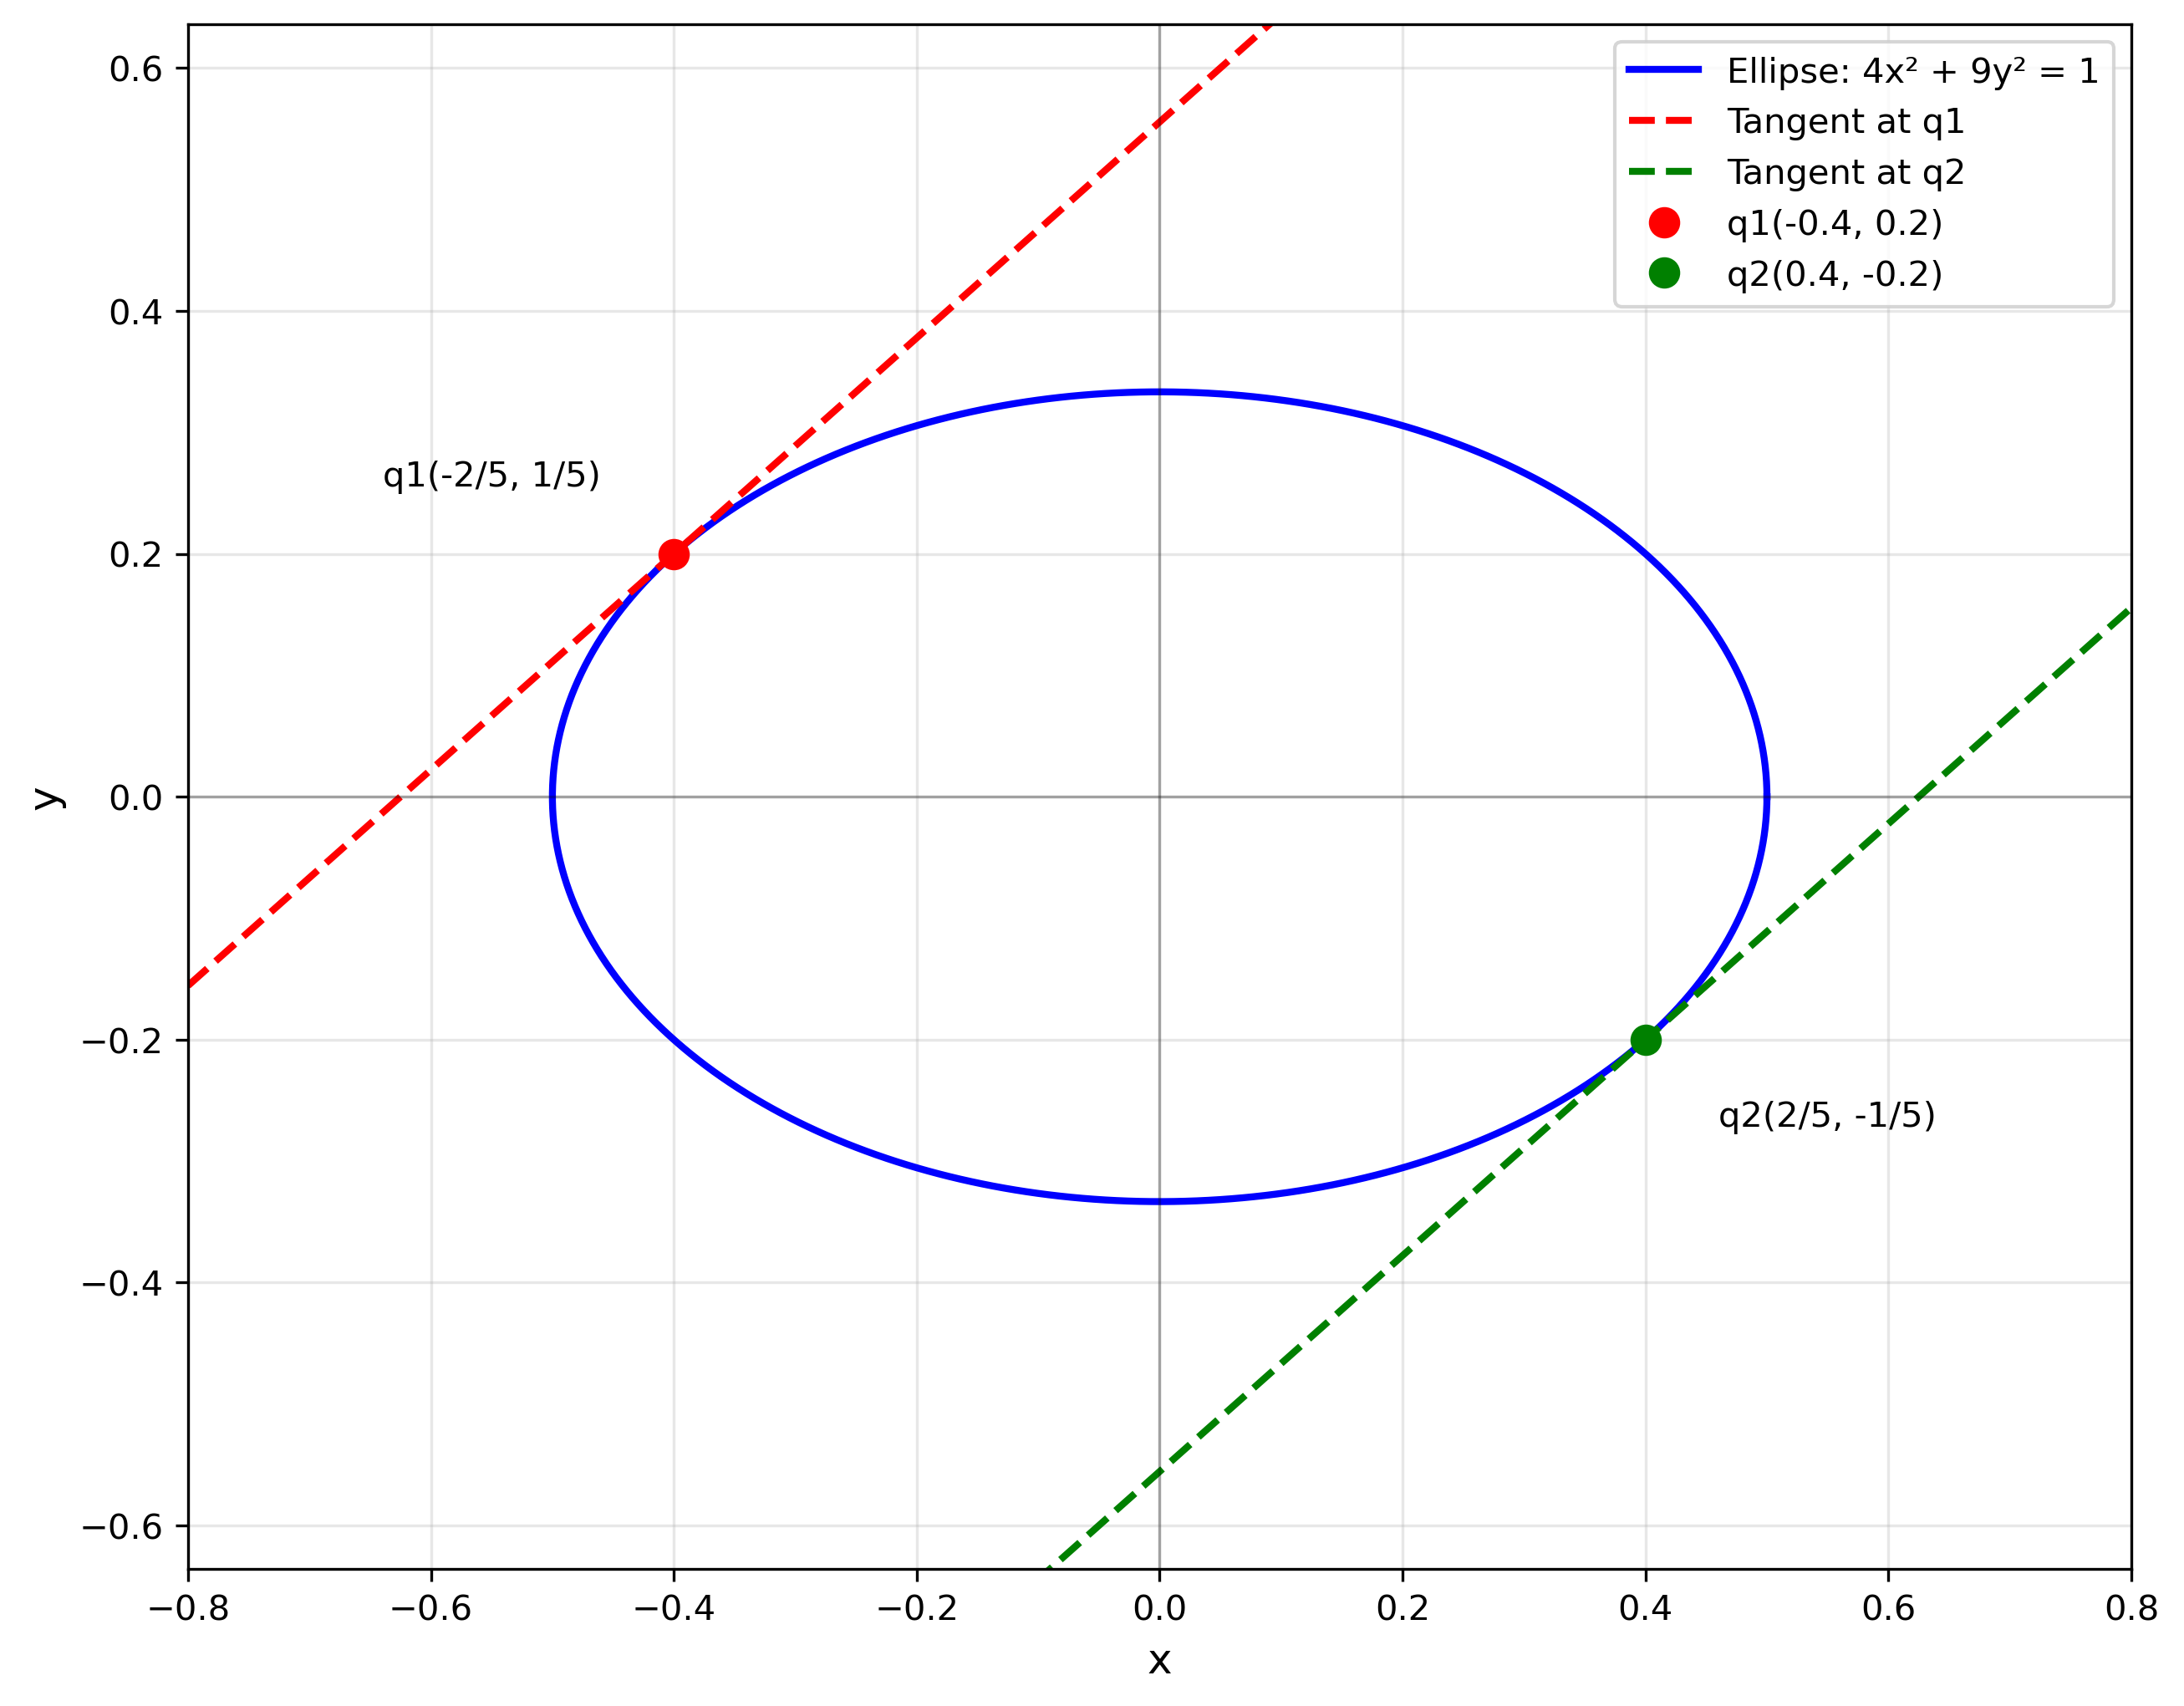
\includegraphics[width=\columnwidth, height=0.8\textheight, keepaspectratio]{figs/fig1.png}
    \label{fig:Beamer/figs/fig1.png}
\end{figure}
\end{frame}

\end{document}